\section{Materiais e Métodos}
\subsection{Escolha da plataforma}
Primeiramente foi feito o estudo do estado da arte das tecnologias utilizadas em coleta de observações da natureza feitas por voluntários \cite{azavea2014, azavea2015}. Com isso, foi possível fazer um levantamento das melhores plataformas existentes hoje. A finalidade deste levantamento foi basear a implementação deste projeto em um já existente e, a partir dele, fazer modificações e otimizações para que atenda às necessidades locais. 

Algumas das plataformas analisadas foram: o \emph{iNaturalist}\footnote{Site do projeto: http://inaturalist.org.}, desenvolvido pela Academia de Ciências da Califórnia, o \emph{Map of Life}\footnote{Site do projeto: http://mol.org.}, desenvolvido pela Universidade Yale, e o \emph{eBird}\footnote{Site do projeto: http://ebird.org.}, desenvolvido pela Universidade Cornell. O iNaturalist foi escolhido como plataforma de desenvolvimento. A escolha foi feita analizando critérios como frequência de atualização do código, uso de software livre, sistema de controle de qualidade de dados utilizado e disponibilidade em vários tipos de dispositivos (desktop, móvel, etc.).

\subsection{Infraestrutura e implantação}
Por se tratar do desenvolvimento e implantação de um sistema já existente, o estudo de recursos exigidos, como a pilha de software\footnote{Conjunto de subsistemas ou componentes de software necessários para criar uma plataforma completa. Isto inclui o sistema operacional, o sistema de banco de dados, o \emph{web server}, a \emph{framework}, dentre outros.} utilizada, serão indispensáveis para garantir a reprodutibilidade do sistema nos servidores do Laboratório de Automação Agrícola -- LAA.

Para hospedagem do website (\emph{back-end}\footnote{Parte de um sistema de computador que não está diretamente acessível ao usuário final, tipicamente responsável pelo armazenamento e manipulação de dados.} e \emph{front-end}\footnote{Parte de um sistema de computador em que o usuário final interage diretamente.}), foi usada uma máquina virtual em um servidor do LAA rodando o Ubuntu 14.04 como sistema operacional e com um endereço de IP público configurado. Além disso, a rede interna da USP foi utilizada para transportar o tráfego externo de dados ao sistema.

Além de configurar o ambiente de produção e implantar o sistema, foi necessário popular o banco de dados com informações iniciais necessárias para o funcionamento do \emph{back-end}, como a árvore taxonômica das espécies.

\subsection{Desenvolvimento}
Por se tratar de sistemas em desenvolvimento paralelo, a sincronização do código entre os projetos é muito importante. Por isso, o GIT\footnote{Sistema de Controle de Versão -- SCV, usado para gerenciamento e automação de códigos.} foi usado para o gerenciamento do código através do serviço Github.com. Este é o mesmo serviço usado pela CalAcademy\footnote{Academia de Ciências da Califórnia.} para manter o projeto iNaturalist.

Para início do desenvolvimento, dois repositórios foram clonados: o principal\footnote{Endereço do repositório: https://github.com/inaturalist/inaturalist.}, com o código-fonte do \emph{back-end} e do \emph{front-end}, e o do aplicativo Android\footnote{Endereço do repositório: https://github.com/inaturalist/iNaturalistAndroid.}. A implementação desta nova versão do iNaturalist foi feita paralelamente com o \emph{upstream}.

Como desenvolvimento desta instânica do iNaturalist foi feito em paralelo com o desenvolvimento do projeto original, o código deste projeto foi periodicamente sincronizado com o projeto original. Esta sincronização foi feita como mostra a figura \ref{fig:git}. 

\begin{figure}[h!]
  \centering
  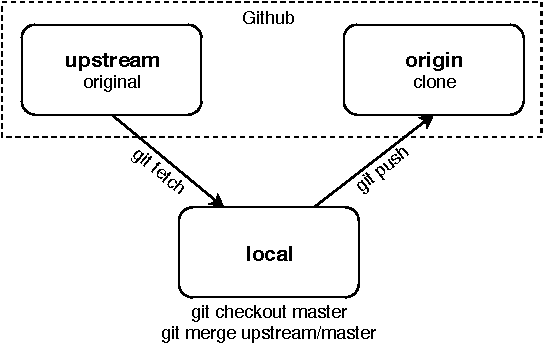
\includegraphics[width=.6\textwidth]{figures/github_diagram.pdf}
  \caption{Diagrama da sincronização do código entre os repositórios.}
  \label{fig:git}
\end{figure}

Como o público álvo é brasileiro, a primeira tarefa foi traduzir todo aplicativo Android para o português. Depois, para incluir recursos de \emph{gamificação} na plataforma, uma nova funcionalidade foi implementada: o sistema de \emph{badges}. Para isto, foram necessárias algumas modificações na estrutura do banco de dados e no código.

% \begin{figure}[h!]
%   \centering
%   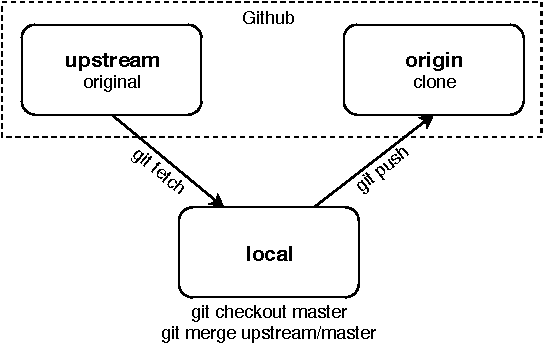
\includegraphics{figures/github_diagram.pdf}
%   \label{fig:github_diagram}
%   \caption{Diagrama de sincronização do código com \emph{upstream}}
% \end{figure}

% Para melhorar a experiência do usuário local com o versão brasileira do iNaturalist, a primeira modificação foi uma tradução completa do aplicativo Android para o português, contando com mais de 200 expressões traduzidas.

% Pensando no gosto do brasileiro por jogos e na estratégia de marketing de gamificacação, que consiste em atribuir ao aplicativo elementos presentes em jogos, como recompensas, foi implementada uma nova função na plataforma iNaturalist que é a recompensa pelas ações dos usuários na rede por um sistema de 'badges'. Cada observação do usuário no iNaturalist contribui para que ele ganhe um novo badge. (Adicionar foto)


% • Tradução completa do app para pt-br (possível pull request)

% • Implementação de 'badges'

% • Árvore taxonômica
